 
\chapter{Population Ordinary Least Squares and Misspecified Linear Model}
 \label{chapter::populationOLS}
 
 Previous chapters assume fixed $X$ and random $Y$. We can also view each observation $(x_i, y_i)$ as IID draws from a population and discuss population OLS. The population OLS allows us to achieve the following goals:
 \begin{enumerate}[label=(G\arabic*), ref=G\arabic*]
 \item
 We can view the OLS from the level of random variables instead of data points. 
 \item
The population OLS  facilitates the discussion of the properties of misspecified linear models.
\item
The population OLS motivates a prediction procedure called {\it conformal prediction} without imposing any distributional assumptions. 
 \end{enumerate}
 
 
 
 

\section{Population OLS}

Assume that $(x_{i},y_{i})_{i=1}^{n}$ are IID with the same distribution
as $(x,y)$, where $x\in\mathbb{R}^{p}$ and $y\in\mathbb{R}$. 
Below I will use $(x,y)$ to denote a general observation, dropping the subscript $i$ for simplicity. 
Let
the joint distribution be $F(x,y)$, and $E(\cdot)$, $\var(\cdot)$,
and $\cov(\cdot)$ be the expectation, variance, and covariance under
this joint distribution. We want to use $x$ to predict $y$.
Theorem \ref{thm::equivalent-definition-of-conditional-mean} below states that the conditional expectation $E(y\mid x)$
is the best predictor in terms of the mean squared error.


\begin{theorem}\label{thm::equivalent-definition-of-conditional-mean}
For any function $m(x)$, we have the decomposition 
\begin{equation}
E\left[\left\{ y-m(x)\right\} ^{2}\right]=E\left[\left\{ E(y\mid x)-m(x)\right\} ^{2}\right]+ E\{ \var(y\mid x) \},\label{eq:decomposition-popols}
\end{equation}
provided the existence of the moments in \eqref{eq:decomposition-popols}. The decomposition \eqref{eq:decomposition-popols} implies
\[
E(y\mid x)=\arg\min_{m(\cdot)}E\left[\left\{ y-m(x)\right\} ^{2}\right]
\]
with the minimum value equaling $E\{ \var(y\mid x)\} ,$ the expectation of the conditional
variance of $y$ given $x$. 
\end{theorem}

 

Theorem \ref{thm::equivalent-definition-of-conditional-mean} is well known in probability theory. I relegate its proof as  Problem \ref{hw11::population-mean}. 
We have finite data points, but the function $E(y\mid x)$ lies in
an infinite dimensional space. Nonparametric estimation of $E(y\mid x)$
is generally a hard problem, especially with a multidimensional $x$.
As a starting point, we often use a linear function of $x$ to approximate
$E(y\mid x)$ and define the population OLS coefficient as
\[
\beta=\arg\min_{b\in\mathbb{R}^{p}} \mathcal{L}(b) ,
\]
where
\begin{align*}
\mathcal{L}(b) & =E\left\{ (y-x^{\T}b)^{2}\right\} \\
 & =E\left\{ y^{2}+b^{\T}xx^{\T}b-2yx^{\T}b\right\} \\
 & =E(y^{2})+b^{\T}E\left(xx^{\T}\right)b-2E\left(yx^{\T}\right)b 
\end{align*}
 is a quadratic function of $b$. From the first-order condition,
we have
\[
\frac{\partial\mathcal{L}(b)}{\partial b}\mid_{b=\beta}=2E\left(xx^{\T}\right)\beta-2E\left(xy\right)=0
\]
based on Proposition \ref{prop::vector-calculus} in Appendix \ref{chapter::linear-algebra}, 
so
\begin{equation}
\label{eq::pols-formula}
\beta= \{ E(xx^{\T}) \} ^{-1}E\left(xy\right) , 
\end{equation}
if $E(xx^{\T})$ is non-degenerate. 
From the second-order condition, 
\[
\frac{\partial^{2}\mathcal{L}(b)}{\partial b\partial b^{\T}}=2E\left(xx^{\T}\right) 
\]
is positive definite. 
So $\beta$ is the unique minimizer of $\mathcal{L}(b)$. 


The above derivation shows that $x^{\T}\beta$ is the best linear predictor. Theorem \ref{thm:bestlinear-conditionalmean} below states  that $x^{\T}\beta$ is
the best linear approximation to the possibly nonlinear conditional mean $E(y\mid x).$
\begin{theorem}
\label{thm:bestlinear-conditionalmean}
If $E(xx^{\T})$ is non-degenerate, then
\begin{eqnarray*}
\beta &=& \arg\min_{b\in\mathbb{R}^{p}}E\left[\left\{ E(y\mid x)-x^{\T}b\right\} ^{2}\right] \\
&=& \{ E(xx^{\T} ) \} ^{-1}E\left\{ xE(y\mid x)\right\} .
\end{eqnarray*}
\end{theorem}
 



As a special case, when the covariate ``$x$'' in the above formulas contains $1$ and a scalar $x$,
the OLS coefficient has the following form.
\begin{corollary}
\label{corollary:scalar-pop-ols}
For scalar $x$ and $y$, we have 
\[
(\alpha,\beta)=\arg\min_{a,b}E(y-a-bx)^{2},
\]
where $\alpha=E(y)-E(x)\beta$ and 
\[
\beta=\frac{\cov(x,y)}{\var(x)} = \rho_{xy} \sqrt{   \frac{\var(y)}{\var(x)}  }
\]
\end{corollary}

Recall that 
$$
\rho_{xy}  = \frac{   \cov(x,y)   }{   \sqrt{   \var(x) \var(y)  }    }
$$
is the population Pearson correlation coefficient. So Corollary \ref{corollary:scalar-pop-ols} gives the population version of the Galtonian formula. 
I leave the proofs of Theorem \ref{thm:bestlinear-conditionalmean} and Corollary \ref{corollary:scalar-pop-ols} as Problems \ref{hw11::condition-mean-app} and \ref{hw11::univariate-ols}.



 
With $\beta$, we can define
\begin{equation}
\varepsilon=y-x^{\T}\beta\label{eq:populationresidualols}
\end{equation}
as the population residual. Because we usually do not use the upper-case letter $E$ for $\varepsilon$, this notation may cause confusion with previous discussion on OLS,  where $\varepsilon$ denotes the vector of the error terms. Here $\varepsilon$ is a scalar in \eqref{eq:populationresidualols}.   
By the definition of $\beta$, we can verify
\begin{equation}
E(x\varepsilon)=E\left\{ x(y-x^{\T}\beta)\right\} =E(xy)-E(xx^{\T})\beta=0.\label{eq:ols-uncorrelated}
\end{equation}
If we include $1$ as a component of $x$, then $E(\varepsilon)=0$,
which, coupled with (\ref{eq:ols-uncorrelated}), implies $\cov(x,\varepsilon)=0$.
So with an intercept in $\beta$, the mean of the population residual
must be zero, and it is uncorrelated with other covariates by construction. 

We can also rewrite (\ref{eq:populationresidualols}) as
\begin{equation}
y=x^{\T}\beta+\varepsilon,\label{eq:population-ols-decomposition}
\end{equation}
which holds by the definition of the population OLS coefficient and residual without any modeling
assumption. We call (\ref{eq:population-ols-decomposition}) with \eqref{eq::pols-formula} and \eqref{eq:populationresidualols} the {\it  population
OLS decomposition}. 


\section{Population FWL Theorem and Cochran's formula}


Assume $(y_i, x_{i1}, x_{i2})_{i=1}^n$ are IID, where $y_i$ is a scalar, $x_{i1}$ has dimension $k$, and $x_{i2}$ has dimension $l$. 
With
$$
x = \begin{pmatrix}
x_1\\
x_2
\end{pmatrix}, 
\quad
\beta = \begin{pmatrix}
\beta_1 \\
\beta_2
\end{pmatrix},
$$
define the population OLS of $y$ on $x_1$ and $x_2$ as
\begin{equation}\label{eq::population-ols-long}
y = \beta^{\T} x =  \beta_1^{\T} x_1 +  \beta_2 ^{\T} x_2+ \varepsilon.
\end{equation}
To aid the interpretation of the population OLS coefficient, we have the following population FWL theorem.


\begin{theorem}
[Population FWL Theorem]
\label{thm::population-fwl}
Consider the population OLS decomposition \eqref{eq::population-ols-long}. 
Define $\tilde{x}_2$ as the residual of the component-wise\footnote{If $x_2$ is a vector, we run population OLS of each component of $x_2$ on $x_1$ to obtain the residual. Vectorize the residuals to obtain $\tilde{x}_2$.} population OLS of $x_2$ on $x_1$:
$$
\tilde{x}_2 = x_2 - E(x_2 x_1^{\T}) E(x_1 x_1^{\T})^{-1} x_1.
$$
Define $\tilde{y}$ as the residual of the population OLS of $y$ on $x_1$:
$$
\tilde{y} = y - E(y x_1^{\T}) E(x_1 x_1^{\T})^{-1} x_1.
$$

Then the coefficient $\beta_2$ has the following equivalent forms:
\begin{eqnarray}
\beta_2 &=&  [ E(xx^{\T})^{-1} E(xy)]_{\textup{the last $l$ components}} \label{eq::population-ols-definition1} \\
&=& E(\tilde{x}_2\tilde{x}_2^{\T})^{-1} E(\tilde{x}_2 y) \label{eq::population-ols-partial1} \\
&=& E(\tilde{x}_2\tilde{x}_2^{\T})^{-1} E(\tilde{x}_2 \tilde{y}) . \label{eq::population-ols-partial2}
\end{eqnarray} 
\end{theorem}

The form \eqref{eq::population-ols-definition1} is the definition of $\beta_2$ from the population OLS \eqref{eq::population-ols-long}. 
The form \eqref{eq::population-ols-partial1} states that $\beta_2$ equals the population OLS coefficient of $y$ on $\tilde{x}_2$. 
The form \eqref{eq::population-ols-partial2} states that $\beta_2$ equals the population OLS coefficient of $\tilde{y}$ on $\tilde{x}_2$. 
\citet{angrist2008mostly} provide a special case of Theorem \ref{thm::population-fwl} with $l=1$.  


\begin{myproof}{Theorem}{\ref{thm::population-fwl}}
Introduce the notation:
$$
E\left( 
\begin{pmatrix}
y\\
x_1\\
x_2
\end{pmatrix}
\begin{pmatrix}
y & x_1^{\T} & x_2^{\T}
\end{pmatrix}
\right) 
= \begin{pmatrix}
E(y^2) & E(y x_1^{\T}) & E(y x_2^{\T}) \\
E(x_1 y) & E(x_1 x_1^{\T}) & E(x_1 x_2^{\T}) \\
E(x_2 y) & E(x_2 x_1^{\T}) & E(x_2 x_2^{\T}) \\
\end{pmatrix}
= \begin{pmatrix}
\Sigma_{00} & \Sigma_{01} & \Sigma_{02} \\
\Sigma_{10} & \Sigma_{11} & \Sigma_{12} \\
\Sigma_{20} & \Sigma_{21} & \Sigma_{22}
\end{pmatrix}.
$$
By definition of the population OLS of $y$ on $x_1$ and $x_2$, we have
$$
\begin{pmatrix}
\beta_1 \\
\beta_2
\end{pmatrix}
= \begin{pmatrix}
\Sigma_{11} & \Sigma_{12} \\
\Sigma_{21} & \Sigma_{22}
\end{pmatrix}^{-1} 
\begin{pmatrix}
\Sigma_{10} \\
\Sigma_{20}
\end{pmatrix}.
$$
Use the first form of the inverse of $2\times 2$ block matrix in Problem \ref{hwmath1::inverse-block-matrix} to obtain
\begin{eqnarray*}
\beta_2 
&=& \begin{pmatrix}
* & *\\
- \Sigma_{22\mid 1}^{-1} \Sigma_{21}  \Sigma_{11}^{-1} & \Sigma_{22\mid 1}^{-1}
\end{pmatrix}
\begin{pmatrix}
\Sigma_{10} \\
\Sigma_{20}
\end{pmatrix} \\
&=& - \Sigma_{22\mid 1}^{-1} \Sigma_{21}  \Sigma_{11}^{-1}  \Sigma_{10} 
+ \Sigma_{22\mid 1}^{-1}\Sigma_{20} \\
&=& \Sigma_{22\mid 1}^{-1} (\Sigma_{20}- \Sigma_{21}  \Sigma_{11}^{-1}  \Sigma_{10} ) , 
\end{eqnarray*}
where $\Sigma_{22\mid 1} = \Sigma_{22} -\Sigma_{21} \Sigma_{11}^{-1} \Sigma_{12} $ and $*$ signifies unimportant terms.



Now we consider the population OLS coefficient of $y$ on $\tilde{x}_2$:
\begin{eqnarray*}
&& E(\tilde{x}_2\tilde{x}_2^{\T})^{-1} E(\tilde{x}_2 y) \\ 
&=& [ E \{  (x_2 - \Sigma_{21} \Sigma_{11}^{-1} x_1) (x_2^{\T} - x_1 ^{\T} \Sigma_{11}^{-1} \Sigma_{12} ) \} ]^{-1}
E\{  (x_2 - \Sigma_{21} \Sigma_{11}^{-1} x_1)  y  \} \\
&=& (\Sigma_{22} -\Sigma_{21} \Sigma_{11}^{-1} \Sigma_{12} )^{-1} (\Sigma_{20} -\Sigma_{21} \Sigma_{11}^{-1} \Sigma_{10} ) \\
&=& \Sigma_{22\mid 1}^{-1}  (\Sigma_{20} -\Sigma_{21} \Sigma_{11}^{-1} \Sigma_{10} )\\
&=& \beta_2.
\end{eqnarray*}

Finally, we consider the population OLS coefficient of $\tilde{y}$ on $\tilde{x}_2$:
\begin{eqnarray*}
&& E(\tilde{x}_2\tilde{x}_2^{\T})^{-1} E(\tilde{x}_2 \tilde{y}) \\
&=& [ E \{  (x_2 - \Sigma_{21} \Sigma_{11}^{-1} x_1) (x_2^{\T} - x_1 ^{\T} \Sigma_{11}^{-1} \Sigma_{12} ) \} ]^{-1}
E\{  (x_2 - \Sigma_{21} \Sigma_{11}^{-1} x_1) (y - x_1 ^{\T} \Sigma_{11}^{-1} \Sigma_{10} ) \} \\
&=& (\Sigma_{22} -\Sigma_{21} \Sigma_{11}^{-1} \Sigma_{12} )^{-1} (\Sigma_{20} -\Sigma_{21} \Sigma_{11}^{-1} \Sigma_{10} ) \\
&=& \Sigma_{22\mid 1}^{-1}  (\Sigma_{20} -\Sigma_{21} \Sigma_{11}^{-1} \Sigma_{10} )\\
&=& \beta_2.
\end{eqnarray*}

\end{myproof}


% correct theorem with x1 and x2 swapped. i want to be coherent with the FWL before
%
%\begin{theorem}
%[Population FWL Theorem]
%\label{thm::population-fwl}
%Consider the population OLS decomposition \eqref{eq::population-ols-long}. 
%Define $\tilde{x}_1$ as the residual of the component-wise\footnote{If $x_1$ is a vector, we run population OLS of each component of $x_1$ on $x_2$ to obtain the residual. Vectorize the residuals to obtain $\tilde{x}_1$.} population OLS of $x_1$ on $x_2$:
%$$
%\tilde{x}_1 = x_1 - E(x_1 x_2^{\T}) E(x_2 x_2^{\T})^{-1} x_2.
%$$
%Define $\tilde{y}$ as the residual of the population OLS of $y$ on $x_2$:
%$$
%\tilde{y} = y - E(y x_2^{\T}) E(x_2 x_2^{\T})^{-1} x_2.
%$$
%
%Then the coefficient $\beta_1$ has the following equivalent forms:
%\begin{eqnarray}
%\beta_1 &=&  [ E(xx^{\T})^{-1} E(xy)]_{\textup{the first $k$ components}} \label{eq::population-ols-definition1} \\
%&=& E(\tilde{x}_1\tilde{x}_1^{\T})^{-1} E(\tilde{x}_1 y) \label{eq::population-ols-partial1} \\
%&=& E(\tilde{x}_1\tilde{x}_1^{\T})^{-1} E(\tilde{x}_1 \tilde{y}) . \label{eq::population-ols-partial2}
%\end{eqnarray} 
%\end{theorem}
%
%
%The form \eqref{eq::population-ols-definition1} is the definition of $\beta_1$ from the population OLS \eqref{eq::population-ols-long}. 
%The form \ref{eq::population-ols-partial1} states that $\beta_1$ equals the population OLS coefficient of $y$ on $\tilde{x}_1$. 
%The form \ref{eq::population-ols-partial2} states that $\beta_1$ equals the population OLS coefficient of $\tilde{y}$ on $\tilde{x}_1$. 
%\citet{angrist2008mostly} provide a special case of Theorem \ref{thm::population-fwl} with $k=1$.  


%\begin{myproof}{Theorem}{\ref{thm::population-fwl}}
%Introduce the notation:
%$$
%E\left( 
%\begin{pmatrix}
%y\\
%x_1\\
%x_2
%\end{pmatrix}
%\begin{pmatrix}
%y & x_1^{\T} & x_2^{\T}
%\end{pmatrix}
%\right) 
%= \begin{pmatrix}
%E(y^2) & E(y x_1^{\T}) & E(y x_2^{\T}) \\
%E(x_1 y) & E(x_1 x_1^{\T}) & E(x_1 x_2^{\T}) \\
%E(x_2 y) & E(x_2 x_1^{\T}) & E(x_2 x_2^{\T}) \\
%\end{pmatrix}
%= \begin{pmatrix}
%\Sigma_{00} & \Sigma_{01} & \Sigma_{02} \\
%\Sigma_{10} & \Sigma_{11} & \Sigma_{12} \\
%\Sigma_{20} & \Sigma_{21} & \Sigma_{22}
%\end{pmatrix}.
%$$
%By definition of the population OLS of $y$ on $x_1$ and $x_2$, we have
%$$
%\begin{pmatrix}
%\beta_1 \\
%\beta_2
%\end{pmatrix}
%= \begin{pmatrix}
%\Sigma_{11} & \Sigma_{12} \\
%\Sigma_{21} & \Sigma_{22}
%\end{pmatrix}^{-1} 
%\begin{pmatrix}
%\Sigma_{10} \\
%\Sigma_{20}
%\end{pmatrix}.
%$$
%Use the second form of the inverse of $2\times 2$ block matrix in Problem \ref{hwmath1::inverse-block-matrix} to obtain
%\begin{eqnarray*}
%\beta_1 
%&=& \begin{pmatrix}
%\Sigma_{11\mid 2}^{-1} &  - \Sigma_{11\mid 2}^{-1} \Sigma_{12}  \Sigma_{22}^{-1} \\
%* & *
%\end{pmatrix}
%\begin{pmatrix}
%\Sigma_{10} \\
%\Sigma_{20}
%\end{pmatrix} \\
%&=& \Sigma_{11\mid 2}^{-1}\Sigma_{10}- \Sigma_{11\mid 2}^{-1} \Sigma_{12}  \Sigma_{22}^{-1}  \Sigma_{20} \\
%&=& \Sigma_{11\mid 2}^{-1} (\Sigma_{10}- \Sigma_{12}  \Sigma_{22}^{-1}  \Sigma_{20} ) , 
%\end{eqnarray*}
%where $\Sigma_{11\mid 2} = \Sigma_{11} -\Sigma_{12} \Sigma_{22}^{-1} \Sigma_{21} $ and $*$ signifies unimportant terms. 
%
%
%Now we consider the population OLS coefficient of $y$ on $\tilde{x}_1$:
%\begin{eqnarray*}
%&& E(\tilde{x}_1\tilde{x}_1^{\T})^{-1} E(\tilde{x}_1 y) \\ 
%&=& [ E \{  (x_1 - \Sigma_{12} \Sigma_{22}^{-1} x_2) (x_1^{\T} - x_2 ^{\T} \Sigma_{22}^{-1} \Sigma_{21} ) \} ]^{-1}
%E\{  (x_1 - \Sigma_{12} \Sigma_{22}^{-1} x_2)  y  \} \\
%&=& (\Sigma_{11} -\Sigma_{12} \Sigma_{22}^{-1} \Sigma_{21} )^{-1} (\Sigma_{10} -\Sigma_{12} \Sigma_{22}^{-1} \Sigma_{20} ) \\
%&=& \Sigma_{11\mid 2}^{-1}  (\Sigma_{10} -\Sigma_{12} \Sigma_{22}^{-1} \Sigma_{20} )\\
%&=& \beta_1.
%\end{eqnarray*}
%
% 
%
%Finally, we consider the population OLS coefficient of $\tilde{y}$ on $\tilde{x}_1$:
%\begin{eqnarray*}
%&& E(\tilde{x}_1\tilde{x}_1^{\T})^{-1} E(\tilde{x}_1 \tilde{y}) \\
%&=& [ E \{  (x_1 - \Sigma_{12} \Sigma_{22}^{-1} x_2) (x_1^{\T} - x_2 ^{\T} \Sigma_{22}^{-1} \Sigma_{21} ) \} ]^{-1}
%E\{  (x_1 - \Sigma_{12} \Sigma_{22}^{-1} x_2) (y - x_2 ^{\T} \Sigma_{22}^{-1} \Sigma_{20} ) \} \\
%&=& (\Sigma_{11} -\Sigma_{12} \Sigma_{22}^{-1} \Sigma_{21} )^{-1} (\Sigma_{10} -\Sigma_{12} \Sigma_{22}^{-1} \Sigma_{20} ) \\
%&=& \Sigma_{11\mid 2}^{-1}  (\Sigma_{10} -\Sigma_{12} \Sigma_{22}^{-1} \Sigma_{20} )\\
%&=& \beta_1.
%\end{eqnarray*}
%\end{myproof}



%\begin{theorem}\label{thm::population-fwl}
%Consider the population OLS decomposition
%\begin{equation}
%y= \beta_0  +  \beta_{1}x_{1}+\cdots+\beta_{p-1}x_{p-1}+\varepsilon \label{eq:popols-componentwise-y}
%\end{equation}
%and the partial population OLS decompositions:
%\begin{eqnarray}
%x_{k}  &=& \gamma_0 +  \gamma_{1}x_{1}+\cdots+x_{k}\text{ excluded } + \cdots +\gamma_{p-1}x_{p-1}+\tilde{x}_{k},\label{eq:popols-x-k} \\
%y &=& \delta_0 +  \delta_{1}x_{1}+\cdots+ x_{k} \text{ excluded } + \cdots +\delta_{p-1}x_{p-1}+\tilde{y}, \label{eq::popols-y} \\
%\tilde{y} &=& \tilde{\beta}_k  \tilde{x}_{k} + \tilde{\varepsilon}, \label{eq::popols-partial}
%\end{eqnarray}
%where $\tilde{x}_{k}$ is the residual from \eqref{eq:popols-x-k} and  $\tilde{y}$ is the residual from \eqref{eq::popols-y}. 
%The coefficient $\beta_{k}$ from \eqref{eq:popols-componentwise-y} equals $  \cov(\tilde{x}_{k},\tilde{y}) / \var(\tilde{x}_{k})$, the coefficient of $\tilde{x}_{k} $ from the population OLS of $\tilde{y}$ on $\tilde{x}_{k}$ in \eqref{eq::popols-partial}, which also equals 
%$
%  \cov(\tilde{x}_{k},y) / \var(\tilde{x}_{k}) , 
%$
%the coefficient of $\tilde{x}_{k} $ from the population OLS of $y$ on $\tilde{x}_{k}$.  Moreover, $\varepsilon $ from \eqref{eq:popols-componentwise-y} equals $\tilde{\varepsilon}$ from \eqref{eq::popols-partial}. 
%\end{theorem}
%
%Similar to the proof of Theorem \ref{thm:fwl}, we can invert the matrix $E(xx^{\T})$ in \eqref{eq::pols-formula} to prove Theorem \ref{thm::population-fwl} directly. Below I adopt an alternative proof which is a modification of the one given by \citet{angrist2008mostly}. 


%\begin{myproof}{Theorem}{\ref{thm::population-fwl}}
%Some basic identities of population OLS help to simplify the proof below. First, the OLS decomposition \eqref{eq:popols-x-k} ensures
%\begin{eqnarray*}
%\cov(\tilde{x}_{k},x_{k})
%  &=& \cov(\tilde{x}_{k},  \gamma_0 +  \gamma_{1}x_{1}+\cdots+ x_{k} \text{ excluded } +\gamma_{p-1}x_{p-1}+\tilde{x}_{k})  \\
%  &=& \cov(\tilde{x}_{k},\tilde{x}_{k})
%\end{eqnarray*}
%that is,
% \begin{equation}
%\cov(\tilde{x}_{k},x_{k}) =\var(\tilde{x}_{k}).  \label{eq::basic1}
% \end{equation}
%It also ensures
%\begin{eqnarray} \label{eq::basic2}
%\cov(\tilde{x}_{k},x_{l}) = 0,\qquad(l\neq k).
%\end{eqnarray}
%Second, the OLS decompositions \eqref{eq:popols-componentwise-y} and (\ref{eq::popols-y}) ensure
%\begin{equation}
%\cov(\tilde{x}_{k},\varepsilon) = 0, \label{eq::basic3}
%\end{equation}
%because $\tilde{x}_{k}$ is a linear combination of $x$ by \eqref{eq:popols-x-k}.  It also ensures 
%\[
%\cov(\tilde{x}_{k}, \delta_0 +  \delta_{1}x_{1}+\cdots+ x_{k} \text{ excluded }   + \cdots  +\delta_{p-1}x_{p-1})=0,
%\]
%which further implies
%\begin{equation}
%\cov(\tilde{x}_{k},y)=\cov(\tilde{x}_{k},\tilde{y}) . \label{eq::basic4}
%\end{equation}
%
% 
%
%
%Now I prove the equivalent forms of the coefficient $\beta_{k}$. 
%From (\ref{eq:popols-componentwise-y}), we have 
%\begin{align*}
%\cov(\tilde{x}_{k},y) & =\cov\left(\tilde{x}_{k}, \beta_0 +  \beta_{1}x_{1}+\cdots+\beta_{p-1}x_{p-1}+\varepsilon\right)\\
% & =\beta_{k} \cov(\tilde{x}_{k},x_{k}) +\sum_{l\neq k}\beta_{l} \cov(\tilde{x}_{k},x_{l}) +\cov(\tilde{x}_{k},\varepsilon) \\
% &= \beta_{k} \var(\tilde{x}_{k}),
%\end{align*}
%by \eqref{eq::basic1}--\eqref{eq::basic3}. 
%Therefore, 
%\[
%\beta_{k}=\frac{\cov(\tilde{x}_{k},y)}{\var(\tilde{x}_{k})} ,
%\]
%which also equals $\tilde{\beta}_k$ by \eqref{eq::basic4}. 
%
%
%Finally, I prove $\varepsilon = \tilde{\varepsilon}$. It suffices to show that $\tilde{\varepsilon} = \tilde{y}  -  \tilde{\beta}_k  \tilde{x}_{k}  $ satisfies
%$$
%E(\tilde{\varepsilon}) = 0, \quad \cov(  x_k, \tilde{\varepsilon} ) = 0,\quad
%\cov( x_l, \tilde{\varepsilon}) = 0\ (l\neq k).
%$$
%The first identity holds by \eqref{eq::popols-partial}. The second identity holds because
%$$
%\cov(  x_k, \tilde{\varepsilon} ) = \cov(x_k,  \tilde{y}) - \tilde{\beta}_k  \cov(x_k, \tilde{x}_{k} )  
%= \cov(\tilde x_k,  \tilde{y}) - \tilde{\beta}_k  \cov(\tilde x_k, \tilde{x}_{k} )  =0
%$$
%by \eqref{eq::basic4}, \eqref{eq::basic1}, and the population OLS of \eqref{eq::popols-partial}. The third identity holds because
%$$
%\cov(  x_l, \tilde{\varepsilon} ) = \cov(x_l,  \tilde{y}) - \tilde{\beta}_k  \cov(x_l, \tilde{x}_{k} )   = 0
%$$
%by \eqref{eq::popols-y} and \eqref{eq::basic2}. 
%\end{myproof}


We also have a population version of Cochran's formula. 
We have the following OLS decompositions of random variables
\begin{eqnarray}
y &=& \beta_1 ^{\T} x_{1} + \beta_2 ^{\T}x_{2} + \varepsilon , \label{eq::long}\\
y&=&\tilde{\beta}_2 ^{\T} x_{2} + \tilde{\varepsilon}, \label{eq::short}\\
x_{1} &=& \delta ^{\T} x_{2} + u . \label{eq::inter}
\end{eqnarray}
Equation \eqref{eq::long} defines the population long regression, and Equation \eqref{eq::short} defines the population short regression. In Equation \eqref{eq::inter}, $\delta$ is a $l \times k$ matrix because it is the OLS decomposition of a vector on a vector. We can view \eqref{eq::inter} as OLS decomposition of each component of $x_{i1}$ on $x_{i2}$. 
Theorem \ref{thm::population-cochran-formula} below states the population version of Cochran's formula.


\begin{theorem}[population Cochran's formula]
\label{thm::population-cochran-formula}
Based on \eqref{eq::long}--\eqref{eq::inter}, we have 
$$
\tilde{\beta}_2 = \beta_2 + \delta \beta_1.
$$
\end{theorem}


I relegate the proof of Theorem \ref{thm::population-cochran-formula} as Problem \ref{hw11::population-cochran}. 



\section{Population $R^2$ and partial correlation coefficient}


Exclude $1$ from $x $ and assume $ x \in \mathbb{R}^{p-1}$ in this subsection. 
Assume that covariates and outcome are centered with mean zero and covariance matrix
\[
\cov\left(\begin{array}{c}
x\\
y
\end{array}\right)=\left(\begin{array}{cc}
\Sigma_{xx} & \Sigma_{xy}\\
\Sigma_{yx} & \sigma_{y}^{2}
\end{array}\right).
\]
There are multiple equivalent definitions of $R^2$. I start with the following definition
\begin{eqnarray}
R^{2}=\frac{\Sigma_{yx}\Sigma_{xx}^{-1}\Sigma_{xy}}{\sigma_{y}^{2}}, \label{eq::r2-population}
\end{eqnarray}
and will give several equivalent definitions below. 
Let $  \beta $ be the
population OLS coefficient of $y$ on $x$, and $\hat{y}=   x^{\T}\beta$ be the best
linear predictor. 
%Let $( E(y),  \beta^{\T} )^{\T}$ be the
%population OLS coefficient of $y$ on $(1,x)$, and $\hat{y}= E(y) +  x^{\T}\beta$ be the best
%linear predictor. 

\begin{theorem}\label{thm::population-r2}
The $R^{2}$ defined in \eqref{eq::r2-population} has the following equivalent forms:
\begin{eqnarray}
R^{2} &=& \frac{\var(\hat{y})}{\var(y)} \label{eq::r2-form1} \\
&=& \max_{b   \in \mathbb{R}^{p-1}  }\rho ^{2}(y,x^{\T}b) \label{eq::r2-form2} \\
&=& \rho ^{2}(y,\hat{y}). \label{eq::r2-form3}
\end{eqnarray}
\end{theorem}

The form \eqref{eq::r2-form1} states that $R^{2}$ equals the ratio of the variance of the best linear predictor of $y$ and the variance of $y$ itself.
The form \eqref{eq::r2-form2} states that $R^{2}$ equals the maximum value of the squared Pearson correlation coefficient between $y$ and a linear combination of $x$, over all possible linear combinations of $x$. 
The form \eqref{eq::r2-form3} states that $R^{2}$ equals the squared Pearson correlation coefficient between $y$ and the best linear predictor of $y$. 

 


\begin{myproof}{Theorem}{\ref{thm::population-r2}}
I first prove \eqref{eq::r2-form1}. 
Because of the centering of $x$, we have $\beta = \Sigma_{xx}^{-1}\Sigma_{xy}$ and 
\begin{align*}
\var(  \hat{y}  ) & =\beta^{\T} \Sigma_{xx} \beta\\
 & = \Sigma_{yx} \Sigma_{xx}^{-1}\Sigma_{xx}\Sigma_{xx}^{-1}\Sigma_{xy}\\
 &= \Sigma_{yx}\Sigma_{xx}^{-1}\Sigma_{xy}. 
\end{align*}
Therefore, $\var(  \hat{y}  ) / \var(y) = R^2$. 

I then prove \eqref{eq::r2-form2}. 
We have 
\[
\rho ^{2}(y,x^{\T}b)=\frac{\text{\cov}^{2}(y,x^{\T}b)}{\var(y)\var(x^{\T}b)}=\frac{b^{\T}\Sigma_{xy}\Sigma_{yx}b}{\sigma_{y}^{2}\times b^{\T}\Sigma_{xx}b}.
\]
Define $\gamma=\Sigma_{xx}^{1/2}b$ and $b=\Sigma_{xx}^{-1/2}\gamma$
such that $b$ and $\gamma$ have one-to-one mapping. So the maximum value of 
\[
\sigma_{y}^{2}\times\rho ^{2}(y,x^{\T}b)=\frac{\gamma^{\T}\Sigma_{xx}^{-1/2}\Sigma_{xy}\Sigma_{yx}\Sigma_{xx}^{-1/2}\gamma}{\gamma^{\T}\gamma} 
\]
equals the maximum eigenvalue of $\Sigma_{xx}^{-1/2}\Sigma_{xy}\Sigma_{yx}\Sigma_{xx}^{-1/2}$, attained when $\gamma$ equals the corresponding eigenvector; see Theorem \ref{theorem::rayleigh} in Appendix \ref{chapter::linear-algebra}. 
The matrix $\Sigma_{xx}^{-1/2}\Sigma_{xy}\Sigma_{yx}\Sigma_{xx}^{-1/2}$ is positive semi-definite and has rank one due to Proposition \ref{eq::matrix-product-inequality} in Appendix \ref{chapter::linear-algebra}, so it has exactly one non-zero eigenvalue which must equal its trace. So
\begin{align*}
\max_{b \in \mathbb{R}^{p-1} }\rho ^{2}(y,x^{\T}b) & =\sigma_{y}^{-2}\text{trace}(\Sigma_{xx}^{-1/2}\Sigma_{xy}\Sigma_{yx}\Sigma_{xx}^{-1/2})\\
 & =\sigma_{y}^{-2}\text{trace}(\Sigma_{xy}\Sigma_{yx}\Sigma_{xx}^{-1/2}\Sigma_{xx}^{-1/2})\\
 & =\sigma_{y}^{-2}\text{trace}(\Sigma_{yx}\Sigma_{xx}^{-1}\Sigma_{xy})\\
 & =\sigma_{y}^{-2}\Sigma_{yx}\Sigma_{xx}^{-1}\Sigma_{xy}\\
 & =R^{2}.
\end{align*}




I finally prove \eqref{eq::r2-form3}. We have
\begin{eqnarray*}
\rho^{2}(y,\hat{y}) &=&
\frac{ \cov(y, \hat{y})^2 }{ \var(y) \var(\hat{y}) } \\
&=& \frac{ \beta^{\T} \Sigma_{xy} \Sigma_{yx} \beta  }{  \sigma_y^2 \Sigma_{yx}\Sigma_{xx}^{-1}\Sigma_{xy} },
\end{eqnarray*}
by the results in the proofs of \eqref{eq::r2-form2} and \eqref{eq::r2-form2}. Use the formula $\beta = \Sigma_{xx}^{-1}\Sigma_{xy}$ to further simplify the above expression as
\begin{eqnarray*}
\rho^{2}(y,\hat{y}) &=&
\frac{ \Sigma_{yx}\Sigma_{xx}^{-1} \Sigma_{xy} \Sigma_{yx} \Sigma_{xx}^{-1}\Sigma_{xy}  }{  \sigma_y^2 \Sigma_{yx}\Sigma_{xx}^{-1}\Sigma_{xy} } \\
&=& \frac{ \Sigma_{yx}\Sigma_{xx}^{-1} \Sigma_{xy}   }{  \sigma_y^2  }  \\
&=& R^2.
\end{eqnarray*}
\end{myproof}



We can also define population partial correlation and $R^{2}.$ For
scalar $y$ and $x$ with another scalar or vector $w$, we can define
the population OLS decomposition based on $(1,w)$ as
\begin{equation}
\label{eq::population-ols-decomposition}
y=\hat{y}+\tilde{y},\qquad x=\hat{x}+\tilde{x},
\end{equation} 
where 
$$ 
 \tilde{y} =  \{ y- E(y) \} - \{ w - E(w) \}^{\T}\beta_{y},\qquad 
 \tilde{x} =  \{ x- E(x) \} - \{  w-E(w) \} ^{\T}\beta_{x} ,
 $$ 
 with $\beta_{y}$ and $\beta_{x}$ being the coefficients of $w$ in these population OLS. 
We then define the population partial correlation coefficient as
\[
\rho_{yx\mid w}=\rho_{\tilde{y}\tilde{x}}.
\]
If the marginal correlation and partial correlation have different signs, then we have Simpson's paradox at the population level. 


With a scalar $w$, we have a more explicit formula below.
\begin{theorem}
\label{thm:populationpartialcorr}For scalar $(y,x,w)$, we have
\[
\rho_{yx\mid w}=\frac{\rho_{yx}-\rho_{xw}\rho_{yw}}{\sqrt{1-\rho_{xw}^{2}}\sqrt{1-\rho_{yw}^{2}}}.
\]
\end{theorem}


I relegate the proof of Theorem \ref{thm:populationpartialcorr} as  Problem \ref{hw11::population-partial-correlation}.


We can also extend the definition of $\rho_{yx\mid w}$ to the partial $R^2$ with a scalar $y$ and possibly vector $x$ and $w$. The population OLS decompositions \eqref{eq::population-ols-decomposition} still hold in the general case. Then we can define the partial $R^2$ between $y$ and $x$ given $w$ as the $R^2$ between $ \tilde{y}$ and $  \tilde{x}$: 
$$
R^2_{y.x|w} = R^2_{ \tilde{y}.  \tilde{x}  } . 
$$



 
 

\section{Inference for the population OLS}


\subsection{Inference with the Eicker--Huber--White standard errors}
Based on the IID data $(x_{i},y_{i})_{i=1}^{n}$, we can
obtain the moment estimator for the population OLS coefficient
\[
\hat{\beta}=\left(n^{-1}\sumn x_{i}x_{i}^{\T}\right)^{-1}\left(n^{-1}\sumn x_{i}y_{i}\right),
\]
and the residuals $ \hat{\varepsilon}_i = y_i - x_i^{\T} \hat{\beta} . $ Assume finite fourth moments of $(x,y)$. We can use the law of large numbers to show that 
\begin{eqnarray*}
n^{-1}\sumn x_{i}x_{i}^{\T} &\rightarrow & E(xx^{\T}), \\
n^{-1}\sumn x_{i}y_{i} &\rightarrow & E(xy) ,
\end{eqnarray*}
so $\hat{\beta}\rightarrow\beta$ in probability. We can use the central limit theorem (CLT) to show that $n^{-1/2}\sumn x_{i}\varepsilon_{i}\rightarrow\N(0,M)$ in distribution, where $M= E(\varepsilon^{2}xx^{\T})$,
so 
\begin{eqnarray}
\label{eq::ols-populationols-clt}
\sqrt{n}(\hat{\beta}-\beta)\rightarrow\N ( 0, V  )
\end{eqnarray}
in distribution, where $V =  B^{-1} M B^{-1}$ with $B =   E(xx^{\T}) $. 
The moment estimator for the asymptotic variance of $\hat{\beta}$ is again
 the Eicker--Huber--White (EHW) robust covariance
estimator:
\begin{eqnarray}
\label{eq::ehw-populationols}
\hat{V}_{\textsc{ehw}} =  
n^{-1}
\left(n^{-1}\sumn x_{i}x_{i}^{\T}\right)^{-1}
\left(n^{-1}\sumn  \hat{\varepsilon}_i^2  x_{i}x_{i}^{\T}\right) 
\left(n^{-1}\sumn x_{i}x_{i}^{\T}\right)^{-1} .
\end{eqnarray}
Following the almost the same proof of Theorem \ref{thm::ehw-fixeddesign-consistency}, we can show that $\hat{V}_{\textsc{ehw}} $ is consistent for the asymptotic covariance $V$. I summarize the formal results below, with the proof relegated as Problem \ref{hw11::population-ols-asymptotics}. 




\begin{theorem}
\label{thm::population-ols}
Assume that $(x_i, y_i)_{i=1}^n \iidsim (x, y)$ with $E ( \| x \|^4 )  <\infty  $ and $E (y^4) <\infty$. We have \eqref{eq::ols-populationols-clt} and $n \hat{V}_{\textsc{ehw}}  \rightarrow  V$ in probability. 
\end{theorem}


So the EHW standard error is not only robust to the heteroskedasticity of the errors but also robust to the misspecification of the linear model \citep{huber::1967, white1980using, angrist2008mostly, buja2019models}. Of course, when the linear model is wrong, we need to modify the interpretation of $\beta$: it is the coefficient of $x$ in the best linear prediction of $y$ or the best linear approximation of the conditional mean function $E(y\mid x)$. 

 
 
\section{To model or not to model?}

\subsection{Population OLS and the restricted mean model}

\begin{figure}[ht]
\centering
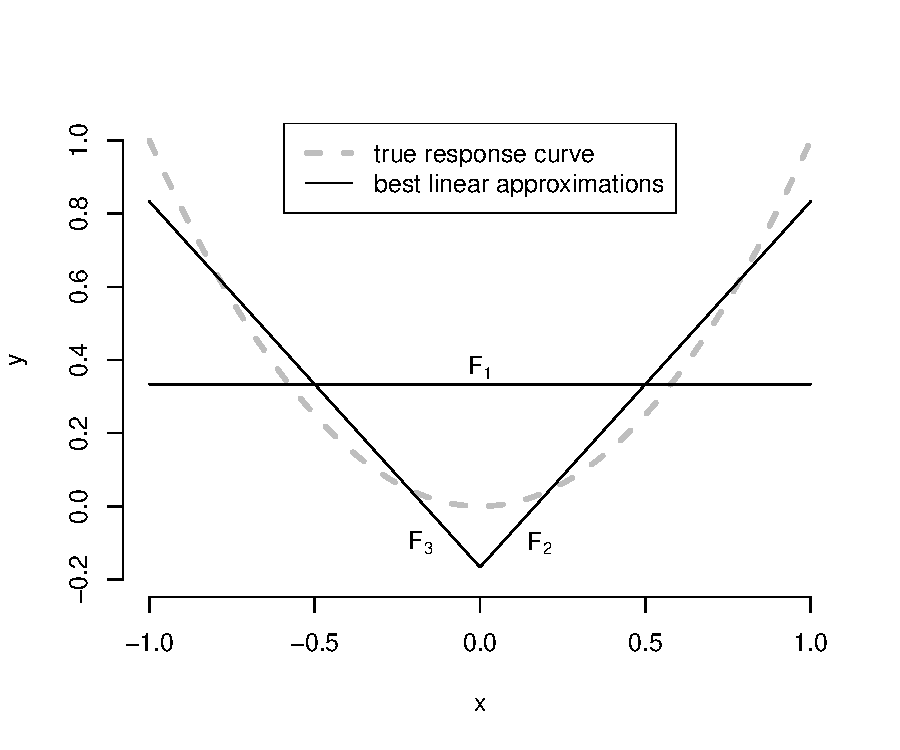
\includegraphics[width = \textwidth]{figures/populationOLS}
\caption{Best linear approximations correspond to three different distributions of $x$.}\label{fig::bestlinearapproximation}
\end{figure}

I start with a simple example. In the following calculation, I will use the fact that the $k$th moment of a Uniform$(0,1)$ random variable equals $1/(k+1)$; see Problem \ref{hwmath2::uniform-moments}.

\begin{example}\label{eg::bestlinearapproximations}
Assume that $x\sim F(x)$, $\varepsilon\sim\N(0,1),x\ind\varepsilon$,
and $y=x^{2}+\varepsilon$.
\begin{enumerate}
\item
If $x\sim F_{1}(x)$ is Uniform$(-1,1)$, then the best linear
approximation is $1/3+0\cdot x$. We can see this result from
$$
\beta(F_{1})=\frac{\text{\cov}(x,y)}{\var(x)}=\frac{\cov(x,x^{2})}{\var(x)}=\frac{E(x^{3})}{\var(x)}=0,
$$
and $\alpha(F_{1})=E(y)=E(x^{2}) =1/3$. 

\item
If $x\sim F_{2}(x)$ is Uniform$(0,1)$, then the best linear approximation is $-1/6+x$. We can see this result from 
$$
\beta(F_{2})=\frac{\cov(x,y)}{\var(x)}=\frac{\cov(x,x^{2})}{\var(x)}=\frac{E(x^{3})-E(x)E(x^{2})}{E(x^{2})-\left\{ E(x)\right\} ^{2}}=\frac{1/4-1/2\times1/3}{1/3-(1/2)^{2}}=1,
$$
and $\alpha(F_{2})=E(y)-\beta E(x)=E(x^{2})-E(x)=1/3-1/2=-1/6$

\item 
If $x\sim F_{3}(x)$ is Uniform$(-1,0)$, then the best linear approximation is $-1/6-x.$ This result holds by symmetry. 
\end{enumerate}
Figure \ref{fig::bestlinearapproximation} shows the true conditional mean function $x^2$ and the best linear approximations. As highlighted in the notation above, the best linear approximation
depends on the distribution of $x$.
\end{example}

 


 

From Example \ref{eg::bestlinearapproximations}, we can see that the best linear approximation depends on the distribution of $X$. This complicates the interpretation of $\beta$ from the population OLS decomposition \citep{buja2019models}. Consequently, this can cause problems for {\it external validity} because $\beta$ will be different in a future environment with different distribution of $X$. \citet[][page 66]{sims2010but} pointed this out as a critique of \citet{angrist2008mostly}.



To ensure the stability of $\beta$ across different environments, we often invoke the following {\it restricted mean model}.

\begin{assumption}[restricted mean model]
\label{assume::model-restricted}
Assume \begin{eqnarray}
E(y\mid x)=x^{\T}\beta
\label{eq::restricted-mean-model}
\end{eqnarray}
or, equivalently, 
\[
y=x^{\T}\beta+\varepsilon,\qquad E(\varepsilon\mid x)=0.
\]
\end{assumption}

Assumption \ref{assume::model-restricted} restricts the conditional mean of $y$ given $x$ to be linear in $x$, justifying the name ``restricted mean model.'' Nevertheless, Assumption \ref{assume::model-restricted} imposes weak assumptions on the distribution of $y$ or $\varepsilon$. 
Under Assumption \ref{assume::model-restricted}, the population OLS coefficient equals the true parameter in the restricted mean model:
\begin{align*}
\left\{ E(xx^{\T})\right\} ^{-1}E(xy) & =\left\{ E(xx^{\T})\right\} ^{-1}E\left\{ xE(y\mid x)\right\} \\
 & =\left\{ E(xx^{\T})\right\} ^{-1}E(xx^{\T}\beta)\\
 & =\beta.
\end{align*}
Moreover, the population OLS coefficient does not depend on the distribution
of $x$. The above asymptotic inference applies to this model too. 


\citet{freedman1981bootstrapping} distinguished two types of OLS as shown in Figure \ref{fig::freedman-classification}: 
\begin{enumerate}[label=(M\arabic*), ref=M\arabic*]
\item
the {\it regression model}, as shown in left-hand side of Figure \ref{fig::freedman-classification};
\item
the {\it correlation model}, as shown in right-hand side of Figure \ref{fig::freedman-classification}. 
\end{enumerate}
In the regression model, we first generate $x$ and $\varepsilon$ under some restrictions, for example, $E(\varepsilon\mid x) = 0$, and then generate the outcome based on $y=x^{\T} \beta + \varepsilon$, a linear function of $x$ with error $\varepsilon$. 
In the correlation model, we start with a pair $(x,y)$, then decompose $y$ into the best linear predictor $x^{\T} \beta $ and the leftover residual $\varepsilon$. 
Compare the subtle difference between the $\varepsilon$ in the regression model and the correlation model. The regression model requires $E(\varepsilon\mid x) = 0$, whereas the correlation model ensures $E(\varepsilon x) = 0$. The regression model imposes a stronger assumption because $E(\varepsilon\mid x) = 0$ implies
$$
E(\varepsilon x) = E\{E(\varepsilon x \mid x)  \} =  E\{E(\varepsilon  \mid x)  x \}  = 0. 
$$

\begin{figure}[th]
\centering
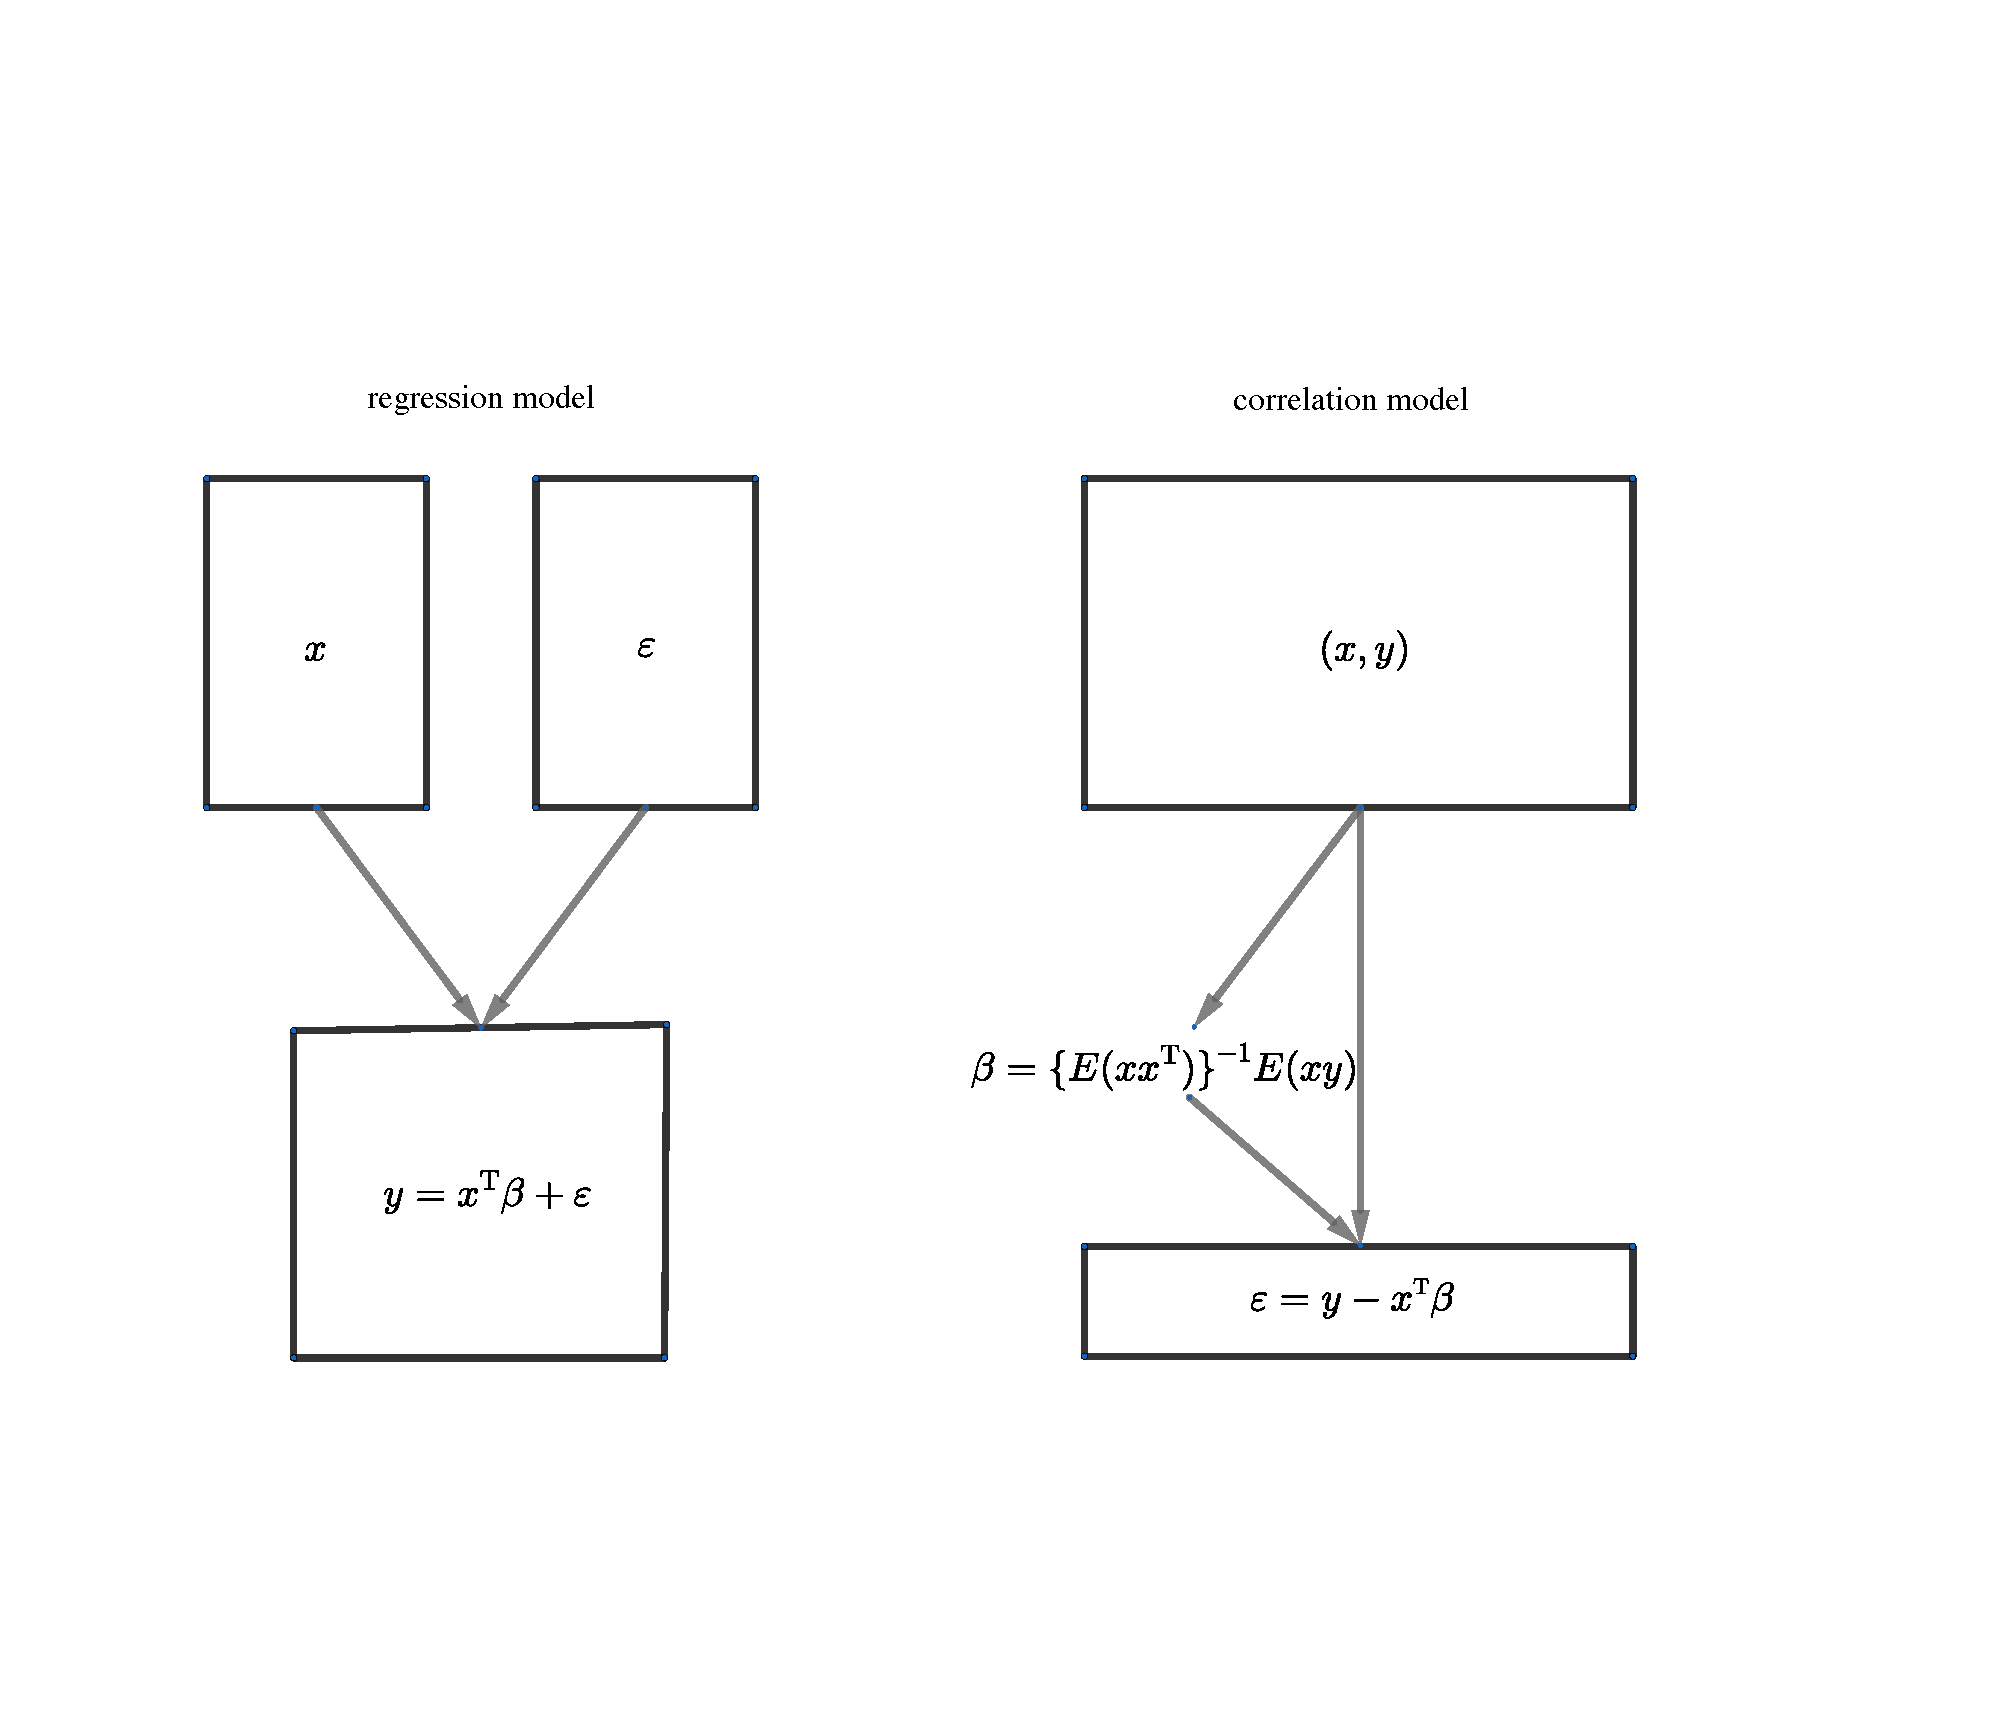
\includegraphics[width = \textwidth]{figures/twoolsfreedman.pdf}
\caption{Freedman's classification of OLS}\label{fig::freedman-classification}
\end{figure}
 



\subsection{More on residual plots}
\label{sec::residual-plot}




Most standard statistical theory for inference assumes a correctly specified linear model (e.g., Gauss--Markov model, Normal linear model, or restricted mean model). However, the corresponding inferential procedures are often criticized since it is challenging to ensure that the model is correctly specified. Alternatively, we can argue that without assuming the linear model, the OLS estimator is consistent for the coefficient in the best linear approximation of the conditional mean function $E(y\mid x)$, which is often a meaningful quantify even the linear model is misspecified. This can be misleading. Example \ref{eg::bestlinearapproximations} shows that the best linear approximation can be a bad approximation to a nonlinear conditional mean function, and it depends on the distribution of the covariates. 



A classic statistical approach is to check whether the residual $\hat\varepsilon_i$ has any nonlinear trend with respect to the covariates. With only a few covariates, we can plot the residual against each covariate; with many covariates, we can plot the residual against the fitted value $\hat{y}_i$. Figure \ref{fig::residual-plots} gives four examples. In these examples, the covariates are the same:
\begin{lstlisting}
n = 200
x1 = rexp(n)
x2 = runif(n)
\end{lstlisting}

The outcome models differ:
\begin{enumerate}
[label=(Y\arabic*), ref=Y\arabic*]
\item\label{modelY1}
linear homoskedastic: 
\ri{y = x1 + x2 + rnorm(n)}; 
\item\label{modelY2}
linear heteroskedastic: 
\ri{y = x1 + x2 + rnorm(n, 0, x1+x2)}; 
\item\label{modelY3}
quadratic homoskedastic: 
\ri{y = x1^2 + x2^2 + rnorm(n)}; 
\item\label{modelY4}
quadratic heteroskedastic: 
\ri{y = x1^2 + x2^2 + rnorm(n, 0, x1+x2)}.
\end{enumerate}



\begin{figure}
\centering
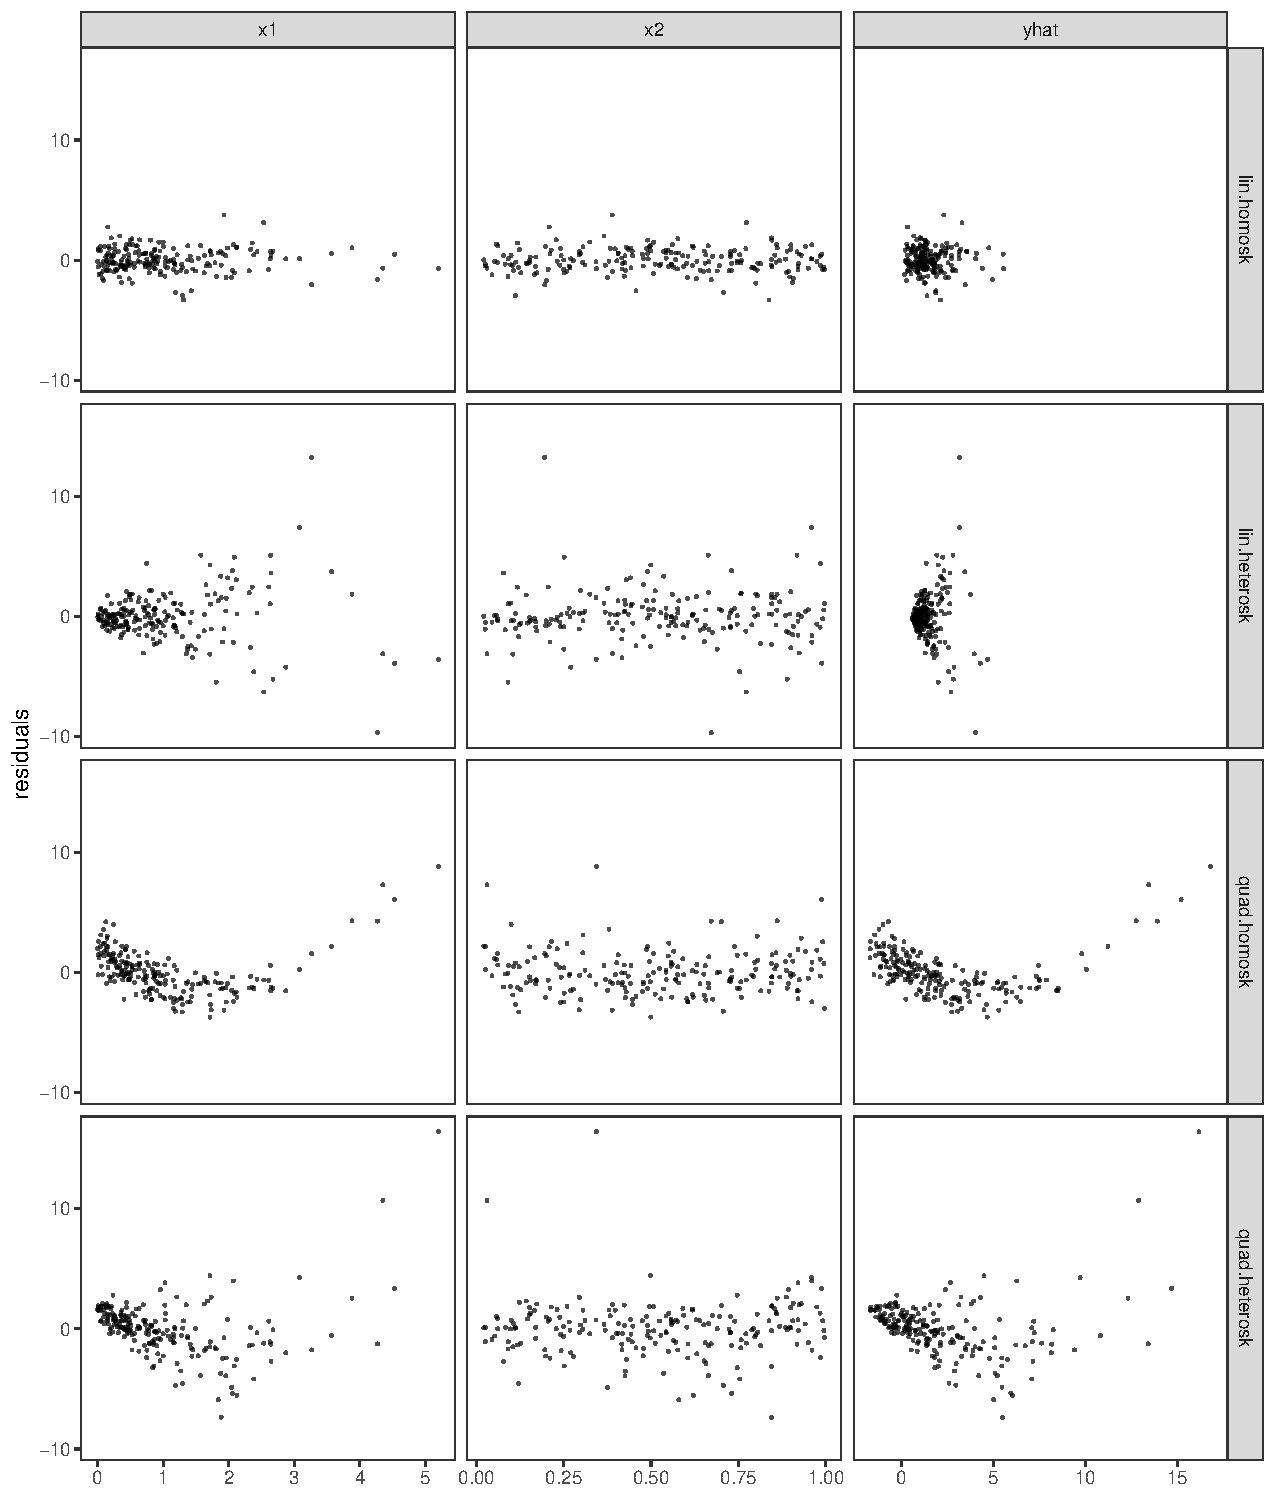
\includegraphics[width = \textwidth]{figures/residualplots.pdf}
\caption{Residual plots}\label{fig::residual-plots}
\end{figure}



In the last two outcome models \eqref{modelY3} and \eqref{modelY4}, the residuals indeed show some nonlinear relationship with the covariates and the fitted value. This suggests that the linear function can be a poor approximation to the true conditional mean function. 



\section{Conformal prediction based on exchangeability}\label{sec::conformal-prediction}


Chapter \ref{sec::prection-normallinear} discusses the prediction of a future outcome $y_{n+1}$ based on $x_{n+1}$ and $(X,Y)$. It requires the Normal linear model assumption. Chapter \ref{chapter::EHW} relaxes the Normality assumption on the error term in statistical inference but does not discuss prediction. Under the heteroskedastic linear model assumption in Chapter \ref{chapter::EHW}, we can predict the mean $E(y_{n+1}) = x_{n+1}^{\T} \beta$ by $x_{n+1}^{\T} \hat\beta$ with asymptotic standard error
$
( x_{n+1}^{\T}  \hat{V}_{\textsc{ehw}}  x_{n+1} )^{1/2},
$
where $ \hat{V}_{\textsc{ehw}}$ is the EHW covariance matrix for the OLS coefficient. However, it is fundamentally challenging to predict $y_{n+1}$ itself since the heteroskedastic linear model allows it to have a completely unknown variance $\sigma^2_{n+1}$. 



Under the population OLS formulation, it seems even more challenging to predict the future outcome since we do not even assume that the linear model is correctly specified. In particular, $x_{n+1}^{\T} \hat\beta$ does not have the same mean as $y_{n+1}$ in general. Perhaps surprisingly, we can construct a prediction interval for $y_{n+1}$ based on $x_{n+1}$ and $(X,Y)$ using an idea called {\it conformal prediction} \citep{vovk2005algorithmic, lei2018distribution}. It leverages the {\it exchangeability}\footnote{Exchangeability is a technical term in probability and statistics. Random elements $z_1, \ldots, z_n$ are exchangeable if $(z_{\pi(1)}, \ldots, z_{\pi(n)} ) $ have the same distribution as $(z_1, \ldots, z_n)$, where $\pi(1), \ldots, \pi(n)$ is a permutation of the integers $1,\ldots, n$. In other words, a set of random elements are exchangeable if their joint distribution does not change under re-ordering. IID random elements are exchangeable.} of the data points 
$$
(x_1, y_1),\ldots,  (x_n, y_n), (x_{n+1}, y_{n+1}) .
$$ 
Pretending that we know the value $y_{n+1} = y^*$, we can fit OLS using $n+1$ data points and obtain residuals
$$
\hat{\varepsilon}_i( y^* ) = y_i - x_i^{\T} \hat{\beta}(  y^* ),\quad (i=1,\ldots, n+1)
$$
where we emphasize the dependence of the OLS coefficient and residuals on the unknown $y^*$. 
The absolute values of the residuals $|\hat{\varepsilon}_i(  y^*  )|$'s are also exchangeable, so the rank of $|\hat{\varepsilon}_{n+1}(  y^*  )|$, denoted by 
$$
\hat{R}_{n+1}(  y^*  )  = 1 +  \sum_{i=1}^{n}  1\{    |\hat{\varepsilon}_{i}(  y^*  )| \leq    |\hat{\varepsilon}_{n+1}(  y^*  )|   \}  ,
$$
must have a uniform distribution over $\{ 1, 2, \ldots,n,n+1 \}$, a known distribution not depending on anything else. It is a pivotal quantity satisfying
\begin{eqnarray}\label{eq::pivotal-conformal}
\pr\left\{   \hat{R}_{n+1}(  y^*   )  \leq \lceil  (1-\alpha)(n+1) \rceil \right\} \geq 1-\alpha.
\end{eqnarray}
Equivalently, this is a statement linking the unknown quantity  $y^*$ and observed data, so it gives a confidence set for $y^*$ at level $1-\alpha$. In practice, we can use a grid search to solve for the inequality \eqref{eq::pivotal-conformal} involving $y^*$. 


%zhichao comment: p = ... no -1?
Below we evaluate the leave-one-out prediction with the Boston housing data. 
\begin{lstlisting}
library("mlbench")
data(BostonHousing)
attach(BostonHousing)
n = dim(BostonHousing)[1]
p = dim(BostonHousing)[2] - 1
ymin = min(medv)
ymax = max(medv)
grid.y  = seq(ymin - 30, ymax + 30, 0.1)
BostonHousing = BostonHousing[order(medv), ]
detach(BostonHousing)

ols.fit.full = lm(medv ~ ., data = BostonHousing,
                  x = TRUE, y = TRUE, qr = TRUE)
beta     = ols.fit.full$coef
e.sigma  = summary(ols.fit.full)$sigma
X        = ols.fit.full$x
Y        = ols.fit.full$y
X.QR     = ols.fit.full$qr
X.Q      = qr.Q(X.QR)
X.R      = qr.R(X.QR)
Gram.inv = solve(t(X.R)%*%X.R)
hatmat   = X.Q%*%t(X.Q) 
resmat   = diag(n) - hatmat
leverage = diag(hatmat)
Resvec   = ols.fit.full$residuals

cvt  = qt(0.975, df = n-p-1)
cvr  = ceiling(0.95*(n+1))

loo.pred = matrix(0, n, 5)
loo.cov  = matrix(0, n, 2)
for(i in 1:n)
{
  beta.i = beta - Gram.inv%*%X[i, ]*Resvec[i]/(1-leverage[i])
  e.sigma.i = sqrt(e.sigma^2*(n - p) - 
                     (Resvec[i])^2/(1 - leverage[i]))/
              sqrt(n - p - 1)
  pred.i = sum(X[i, ]*beta.i) 
  lower.i = pred.i - cvt*e.sigma.i/sqrt(1 - leverage[i])
  upper.i = pred.i + cvt*e.sigma.i/sqrt(1 - leverage[i])
  loo.pred[i, 1:3] = c(pred.i, lower.i, upper.i)
  loo.cov[i, 1] = findInterval(Y[i], c(lower.i, upper.i))
  
  grid.r  = sapply(grid.y,
                   FUN = function(y){
                     Res = Resvec + resmat[, i]*(y - Y[i]) 
                     rank(abs(Res))[i]
                   })
  Cinterval = range(grid.y[grid.r<=cvr])
  loo.pred[i, 4:5] = Cinterval
  loo.cov[i, 2] = findInterval(Y[i], Cinterval)
  
}
\end{lstlisting}

In the above code, I use the QR decomposition to compute $X^{\T} X$ and $H$. Moreover, the calculations of \ri{lower.i}, \ri{upper.i}, and \ri{Res} use some tricks to avoid fitting $n$ OLS. I relegate the justification of them to Problem \ref{hw11::loo-conformal}. 

The variable \ri{loo.pred} has five columns corresponding to the point predictors, lower and upper intervals based on the Normal linear model and conformal prediction. 
% zhichao comment: Normal model or Gauss-Markov? -- Normal linar model
\begin{lstlisting}
> colnames(loo.pred) = c("point", "G.l", "G.u", "c.l", "c.u")
> head(loo.pred)
         point        G.l       G.u   c.l  c.u
[1,]  6.633514  -2.941532 16.208559  -3.5 16.7
[2,]  8.806641  -1.349367 18.962649  -2.6 20.1
[3,] 12.044154   2.608290 21.480018   2.2 21.8
[4,] 11.025253   1.565152 20.485355   1.2 21.0
[5,] -5.181154 -14.819041  4.456733 -15.0  4.9
[6,]  8.324114  -1.382910 18.031138  -2.0 18.8
\end{lstlisting}

Figure \ref{fig::pi-boston-housing-conformal} plots the observed outcomes and the prediction intervals for the 20 observations with the outcomes at the bottom, middle, and top. The Normal and conformal intervals are almost indistinguishable. For the observations with the highest outcome, the predictions are quite poor. Surprisingly, the overall coverage rates across observations are close to $95\%$ for both methods. 
\begin{lstlisting}
> apply(loo.cov==1, 2, mean)
[1] 0.9486166 0.9525692
\end{lstlisting}

Figure \ref{fig::ratio-boston-housing-conformal} compares the lengths of the two prediction intervals. Although the conformal prediction intervals are slightly wider than the Normal prediction interval, the differences are rather small, with the ratio of the length above 0.96.


\begin{figure}
\centering
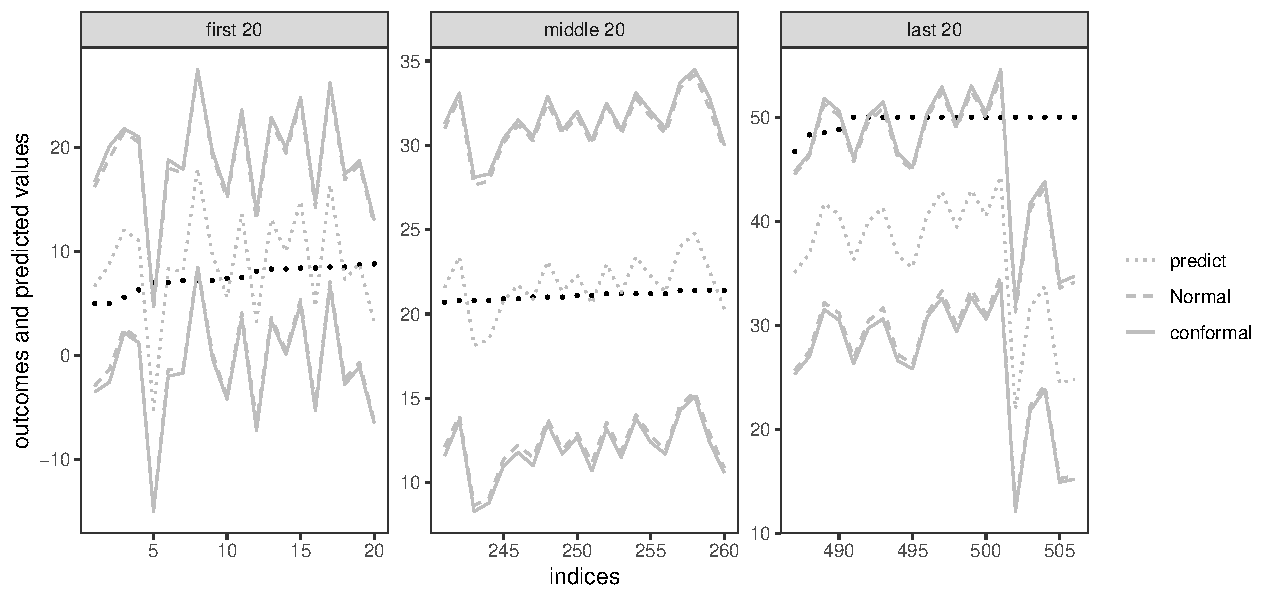
\includegraphics[width = 0.95\textwidth]{figures/GCprediction_intervals.pdf}
\caption{Leave-one-out prediction intervals based on the Boston housing data.
The left, middle and right panels are for the 20 observations with the outcomes at the bottom, middle, and top, respectively.
Each panel shows the original outcomes, predicted outcomes, as well as the prediction intervals based on the Normal linear model and conformal prediction. 
}\label{fig::pi-boston-housing-conformal}
\end{figure}




\begin{figure}
\centering
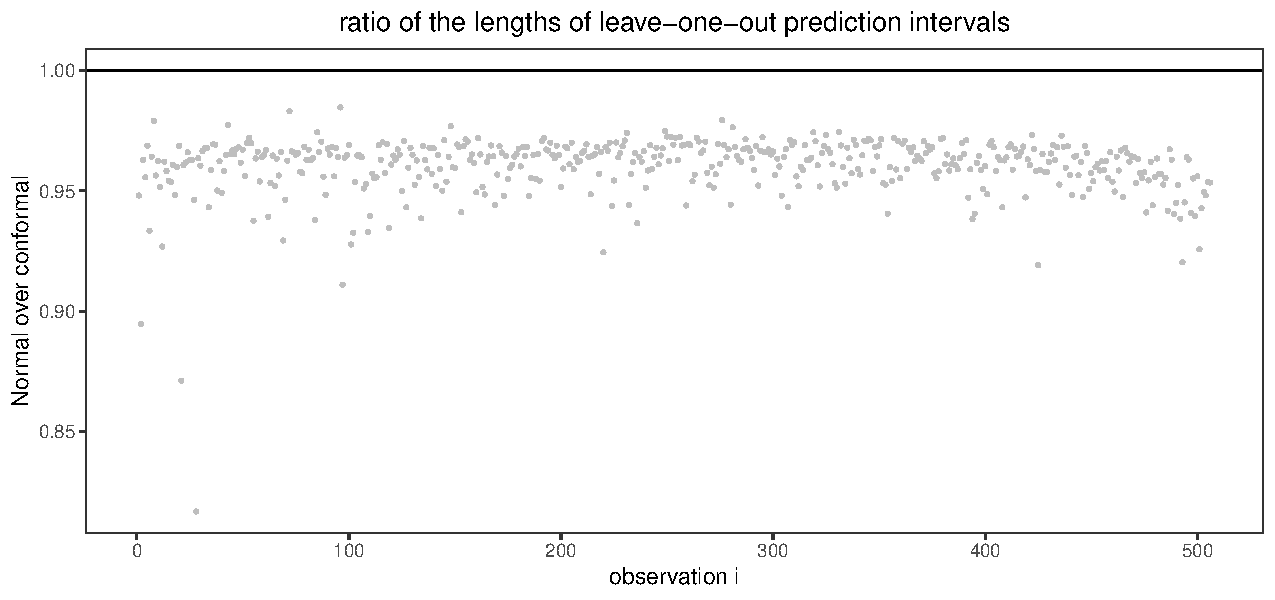
\includegraphics[width = 0.95\textwidth]{figures/GaussianConformalLOOpred.pdf}
\caption{Boston housing data}\label{fig::ratio-boston-housing-conformal}
\end{figure}


 
If you read the above argument for conformal prediction again, you will realize that the whole argument does not rely on using OLS as the predictor. You can replace OLS with an arbitrary predictor, without harming the theoretical guarantee of the conformal prediction interval. Conformal prediction is a powerful idea for using black-box predictors while maintaining confidence interval guarantees. See \citet{angelopoulos2023conformal} for its recent developments and applications.



Nevertheless, the confidence interval guarantees based on conformal prediction differ from that based on the Normal linear model. In particular, the conformal prediction interval covers $y_{n+1}$ with probability larger than or equal to $1-\alpha$, {\it averaged} over the randomness of the past data and future $x_{n+1}$, whereas the prediction interval based on the Normal linear model covers $y_{n+1}$ with probability larger than or equal to $1-\alpha$, {\it conditional} on all observed covariates. 
Therefore, the magic of conformal prediction comes from modifying the statistical model and the theoretical guarantees. 
Some practitioners may argue that the conditional coverage guarantee is more relevant than the average coverage guarantee. In those cases, the conformal prediction interval should be used with caution. 



\section{Homework problems}

\paragraph{Conditional mean}\label{hw11::population-mean}

Prove Theorem \ref{thm::equivalent-definition-of-conditional-mean}. 

\paragraph{Best linear approximation}\label{hw11::condition-mean-app}

Prove Theorem \ref{thm:bestlinear-conditionalmean}.

Remark: It is similar to Problem \ref{hw7::sample-partial-correlation}.

\paragraph{Univariate population OLS}\label{hw11::univariate-ols}

Prove Corollary \ref{corollary:scalar-pop-ols}.

\paragraph{Asymptotics for the population OLS}\label{hw11::population-ols-asymptotics}

Prove Theorem \ref{thm::population-ols}. 


\paragraph{Population Cochran's formula}\label{hw11::population-cochran}

Prove Theorem \ref{thm::population-cochran-formula}. 


\paragraph{Canonical correlation analysis (CCA)}\label{hw11::cca}

Assume that $(x,y)$, where $x \in \mathbb{R}^p$ and $y \in \mathbb{R}^k$, has the joint non-degenerate covariance matrix:
$$
\begin{pmatrix}
\Sigma_{xx} & \Sigma_{xy} \\
\Sigma_{yx} & \Sigma_{yy}
\end{pmatrix}. 
$$
\begin{enumerate}
\item
Find the best linear combinations $(\alpha, \beta)$ that
give the maximum Pearson correlation coefficient:
\[
(\alpha, \beta) = 
\text{\ensuremath{\arg\max_{a \in \mathbb{R}^k ,  b \in \mathbb{R}^p}}}\ \rho(y^{\T}a,x^{\T}b).
\]
Note that you need to detail the steps in calculating $(\alpha, \beta)$ based on the covariance matrix above.

\item
Define the maximum value as $\textsc{cc}(x,y)$. Prove that $\textsc{cc}(x,y) \geq 0$, and $\textsc{cc}(x,y) = 0$ if $x\ind y$. 
\end{enumerate}

Remark: The maximum value $\textsc{cc}(x,y)$ is called the canonical correlation between $x$ and $y$. 
We can also define partial canonical correlation between $x$ and $y$ given $w$.

\paragraph{Population partial correlation coefficient}\label{hw11::population-partial-correlation}

Prove Theorem \ref{thm:populationpartialcorr}. 




\paragraph{Independence and correlation}\label{hw11::independence-correlation}

With scalar random variables $x$ and $y$, it is well known that if $x\ind y$, then $\rho_{yx}=0$. However, with another random variable $w$, if $x\ind y\mid w$, then $\rho_{yx\mid w}=0$ may not hold. 

Give a counterexample in which  $x\ind y\mid w$ but $\rho_{yx\mid w}\neq 0$.


Remark: 
With scalar random variables $x$ and $y$, if $x\ind y$, then we have $\cov(y, x) = 0$,  which implies 
$$
\rho_{yx}=  \frac{ \cov(y, x)  }{ \sqrt{   \var(y)  \var(x)   }  } = 0.
$$
With another random variable $w$, if $x\ind y\mid w$, then we have $\cov(y, x\mid w) = 0$, which, however, does not imply $\rho_{yx\mid w}=0$ because $\rho_{yx\mid w}$ is not defined as 
$$
\frac{ \cov(y, x\mid w)  }{ \sqrt{   \var(y\mid w)  \var(x\mid w)   }  }. 
$$
\citet{shah2020hardness} had related discussion on this issue. 




\paragraph{Best linear approximation of a cubic curve}\label{hw11::bestlinear-cubic}

Assume that $x\sim\N(0,1)$, $\varepsilon\sim\N(0,\sigma^{2})$, $x\ind\varepsilon$,
and $y=x^{3}+\varepsilon$. Find the best linear approximation of
$E(y\mid x)$ based on $(1, x)$.  Plot both $E(y\mid x)$ and its best linear approximation together and compare them. 

 
 

\paragraph{Leave-one-out formula in conformal prediction}\label{hw11::loo-conformal}

Justify the calculations of \ri{lower.i}, \ri{upper.i}, and \ri{Res} in Section \ref{sec::conformal-prediction}. 




\paragraph{Conformal prediction for multiple outcomes}
Assuming exchangeability of 
$$
(x_1,y_1),\ldots,  (x_n,y_n), (x_{n+1},y_{n+1}), \ldots , (x_{n+k},y_{n+k}).   
$$
Propose a method to construct joint conformal prediction regions for $(y_{n+1},\ldots, y_{n+k})$ based on $(X,Y)$ and $(x_{n+1},\ldots, x_{n+k})$.





\paragraph{Cox's theorem}\label{hw11::cox-theorem1960}


\citet{cox1960jrssb} considered the data-generating process
$$
x_1 \longrightarrow x_2  \longrightarrow y
$$
under the following linear models:
for $i=1,\ldots, n$, we have 
$$
x_{i2} = \alpha_0 + \alpha_1x_{i1} + \eta_i
$$
and
$$
y_i = \beta_0 + \beta_1 x_{i2} + \varepsilon_i
$$
where $\eta_i$ has mean 0 and variance $\sigma_\eta^2$, $\varepsilon_i$ has mean 0 and variance $\sigma_\varepsilon^2$, and the $\eta_i$s and  $\varepsilon_i$s are independent.
The linear model implies
$$
y_i = (\beta_0 + \beta_1\alpha_0) + (\beta_1 \alpha_1) x_{i1} +   (\varepsilon_i  +  \beta_1  \eta_i  )
$$
where $\varepsilon_i  +  \beta_1  \eta_i$s are independent with mean 0 and variance $\sigma_\varepsilon^2 + \beta_1^2 \sigma_\eta^2$. 

Therefore, we have two ways to estimate $\beta_1 \alpha_1$:
\begin{enumerate}[label=(W\arabic*), ref=W\arabic*]
\item
the first estimator is $\hat\gamma_1$,  the OLS estimator of the $y_i$'s on the $x_{i1}$'s with the intercept; 

\item
the second estimator is $\hat\alpha_1 \hat\beta_1$, the product of the OLS estimator of the $x_{i2}$'s on the $x_{i1}$'s with the intercept and that of the $y_i$'s on the $x_{i2}$'s with the intercept. 
\end{enumerate}

\citet{cox1960jrssb} reported Theorem \ref{thm::cox-theorem-1960} below. Prove Theorem \ref{thm::cox-theorem-1960}. 

\begin{theorem}
\label{thm::cox-theorem-1960}
Let $X_1 = (x_{11}, \ldots, x_{n1})$. 
We have 
$$
\var(\hat\alpha_1 \hat\beta_1 \mid X_1) \leq \var(\hat\gamma_1\mid X_1) ,
$$
and more precisely,
$$
\var(\hat\gamma_1\mid X_1) 
= \frac{   \sigma_\varepsilon^2     + \beta_1^2  \sigma_\eta^2   }{    \sum_{i=1}^n   (x_{i1} - \bar{x}_1)^2     }
$$
and
$$
\var(\hat\alpha_1 \hat\beta_1 \mid X_1) 
= \frac{   \sigma_\varepsilon^2   E(  \hat\rho_{12}^2 \mid X_1)   + \beta_1^2  \sigma_\eta^2   }{    \sum_{i=1}^n   (x_{i1} - \bar{x}_1)^2     }
$$
where $\hat\rho_{12} \in [-1,1]$ is the sample Pearson correlation coefficient between the $x_{i1}$'s and the $x_{i2}$'s. 
\end{theorem}

 

Remark: If we further assume that the error terms are Normal, then $\hat\alpha_1 \hat\beta_1$ is the maximum likelihood estimator for $\alpha_1 \beta_1$. Therefore, the asymptotic optimality theory for the maximum likelihood estimator justifies the superiority of $\hat\alpha_1 \hat\beta_1$ over $\hat\gamma_1$. Theorem \ref{thm::cox-theorem-1960} provides a stronger finite-sample result without assuming the Normality of the error terms. 



\paragraph{Measurement error and Frisch's bounds}\label{hw11::measurement-error}



\begin{enumerate}
\item
Given scalar random variables $x$ and $y$, we can obtain the population OLS coefficient $(\alpha, \beta)$ of $y$ on $(1,x)$. However, $x$ and $y$ may be measured with errors, that is, we observe $x^* = x + u$ and $y^* = y + v$, where $u$ and $v$ are mean zero error terms satisfying $u\ind v$  and $(u ,v )\ind (x,y)$. We can obtain the population OLS coefficient $(\alpha^*, \beta^*)$ of $y^*$ on $(1,x^*)$ and the population OLS coefficient $(a^*, b^*)$ of $x^*$ on $(1,y^*)$. 

 Prove that if $\beta = 0$ then $ \beta^*  =b^* = 0 $; if $\beta \neq  0$ then
%$$
%\beta^* = \beta \frac{  \var(x) }{  \var(x) + \var(u) }
%$$
%and 
$$ 
| \beta^* | \leq |\beta | \leq 
1 / |  b^* |   .
$$





\item
Given scalar random variables $x, y$ and a random vector $w$, we can obtain the population OLS coefficient $(\alpha, \beta, \gamma)$ of $y$ on $(1,x,w)$. When $x$ and $y$ are measured with error as above with mean zero errors satisfying $u\ind v$ and  $(u ,v )\ind (x,y,w)$, we can obtain the population OLS coefficient $(\alpha^*, \beta^*, \gamma^*)$ of $y$ on $(1,x^*,w)$, and the population OLS coefficient $(a^*, b^*, c^*)$ of $x^*$ on $(1,y^*,w)$.

Prove that the same result holds as in the first part of the problem. 
\end{enumerate}




Remark: \citet{tamer2010partial} reviewed \citet{frisch1934statistical}'s upper and lower bounds for the univariate OLS coefficient based on the two OLS coefficients of the observables. The second part of the problem extends the result to the multivariate OLS with a covariate subject to measurement error. The lower bound is well documented in most books on measurement errors, but the upper bound is much less well known. 




\paragraph{A three-way decomposition}\label{hw11::three-way-ols}

The main text of this chapter focuses on the two-way decomposition of the outcome:
$
y = x^{\T} \beta + \varepsilon ,
$
where $\beta$ is the population OLS coefficient and $\varepsilon$ is  the population OLS residual. However, $x^{\T} \beta$ is only the best linear approximation to the true conditional mean function $\mu(x) =  E(y \mid x)$. This suggests the following three-way decomposition of the outcome:
$$
y = x^{\T} \beta  + \{ \mu(x)  - x^{\T} \beta \} + \{ y -  \mu(x) \},
$$
which must hold without any assumptions. Introduce the notation for the linear term 
$$
\hat{y} = x^{\T} \beta,
$$ 
 the notation for the approximation error:
$$
\delta = \mu(x)  - x^{\T} \beta ,
$$
and the notation for the
 ``ideal residual'':
$$
e =  y -  \mu(x) .
$$
Then 
we can decompose the outcome as
$$
y = \hat{y}   +   \delta  + e
$$
and
 the population OLS residual as
$$
 \varepsilon  =  \{ \mu(x)  - x^{\T} \beta \} + \{ y -  \mu(x) \} =  \delta  + e. 
$$


\begin{enumerate}
\item
Prove  
$$
E(   \hat{y}    e \mid x ) = 0,\quad
E(   \delta   e \mid x ) = 0
$$
and
$$
E(   \hat{y}    e  ) = 0,\quad
E(   \delta   e   ) = 0,\quad
E(  \hat{y}   \delta  ) = 0.
$$
Prove
$$
E( \varepsilon^2 ) = E(  \delta ^2 ) + E(  e^{2}) . 
$$

\item
%Recall the formula of the population OLS coefficient
%$$
%\beta =  \{ E(xx^{\T})  \}^{-1}  E(xy)
%$$
%and the formula of the OLS coefficient
%$$
%\hat{\beta} = \left( n^{-1} \sumn x_i x_i^{\T}  \right)^{-1}  \left( n^{-1} \sumn x_i y_i  \right).
%$$
Introduce an intermediate quantity between the population OLS coefficient $\beta $ and the OLS coefficient $\hat{\beta} $:
$$
\tilde{\beta} = \left( n^{-1} \sumn x_i x_i^{\T}  \right)^{-1}  \left( n^{-1} \sumn x_i \mu(x_i)  \right).
$$
Equation \eqref{eq::ols-populationols-clt} states that 
$
\sqrt{n} (  \hat{\beta}  - \beta ) \rightarrow \N(0,  B^{-1} M B^{-1} )
$
in distribution, 
where $B = E(xx^{\T})$ and $M = E(\varepsilon^2 xx^{\T})$. 


Prove that 
$$
\cov( \hat{\beta}  - \beta ) = \cov(  \hat{\beta}  - \tilde\beta ) + \cov(   \tilde\beta - \beta  ),
$$
and moreover, 
\begin{eqnarray*}
\sqrt{n} (  \hat{\beta}  - \tilde\beta ) & \rightarrow & \N(0,  B^{-1} M_1 B^{-1} ),\\ 
\sqrt{n} (    \tilde\beta - \beta )  & \rightarrow & \N(0,  B^{-1} M_2 B^{-1} )
\end{eqnarray*}
in distribution, where 
\begin{eqnarray*}
M_1 &=& E(e^{2} xx^{\T}),\\ 
M_2 &=& E( \delta^2 xx^{\T})
\end{eqnarray*}
Verify that $M = M_1 + M_2$. 
\end{enumerate}


Remark: To prove the result, you may find the law of total covariance formula in \eqref{theorem::law-total-cov} helpful. We can also write $M_1$ as $M_1 = E\{ \var(y\mid x) xx^{\T} \}$. So the meat matrix $M$ has two sources of uncertainty, one is from the conditional variance of $y$ given $x$, and the other is from the approximation error. 
 
 
